\documentclass[12pt]{article}

\usepackage[paperwidth=120cm
    , paperheight=150cm
    , landscape
    , top=8cm
    , bottom=5cm
    , right=10cm
    , left=10cm
    ]{geometry}

\usepackage{graphicx}
\usepackage{standalone}
\usepackage{amsmath}
%\usepackage[T1]{fontenc}
\usepackage{avant}
\usepackage{lmodern}
\usepackage{tikz}
\usepackage{tikzscale}
\usepackage{enumitem}
\usetikzlibrary{shapes,arrows,positioning}
\usetikzlibrary{arrows.spaced}
\usetikzlibrary{decorations.text}
\usetikzlibrary{spy,calc,fit}
\usetikzlibrary{shapes.arrows}

\usepackage{color}
\usepackage{moresize}
\usepackage{lipsum} % dummy text
\usepackage{multicol}

\pgfdeclarelayer{background}
\pgfdeclarelayer{layer1}
\pgfdeclarelayer{layer2}
\pgfdeclarelayer{layer3}
\pgfdeclarelayer{foreground}

% This macro creates header.
\newcommand{\HEADING}[1]
{
    \tikz \path[] 
        % node {\includegraphics[scale=0.3]{./images/heading.png}}
        node [right] {\fontsize{2.5cm}{1cm}\selectfont
            \textcolor{black}{\hspace{1cm}#1}
        };
    \\
}

\newcommand{\SECTION}[1]
{
    \vspace{0.5cm}
    \tikz \path[] 
        %node {\includegraphics[scale=0.2]{./images/heading.png}}
        node [right] {\fontsize{1.8cm}{1cm}\selectfont
            \textcolor{blue}{\hspace{1cm}#1}
        };
        \par
}

\newcommand{\CAPTION}[1]
{
    {\fontsize{1.2cm}{1cm}\fontfamily{\sfdefault}\selectfont {\textcolor{black}{#1}}\par}
}

\newcommand{\TEXT}[1]
{
   { \fontsize{1.4cm}{1.0cm}\fontfamily{\sfdefault}\selectfont {#1}\par }
}

\newcommand{\ITEM}[1]
{
    {\fontsize{1cm}{1.0cm}\fontfamily{\sfdefault}\selectfont {#1}\par }
}

\newcommand{\MOOSE}[0]{\textsc{\textcolor{black}{MOOSE}}}

\newcommand{\MOOSELOGO}[0]{
    \tikz \node[inner sep=1mm] {\includegraphics[scale=0.6]{./images/moose_logo_tiny.png}}; 
}

\renewcommand{\labelitemi}{{\Huge$\bullet$}}

\newenvironment{Figure}
  {\par\medskip\noindent\minipage{\linewidth}}
  {\endminipage\par\medskip}

\tikzset{
  every overlay node/.style={
    draw=black,fill=white,rounded corners,anchor=north west,
  },
}
% Usage:
% \tikzoverlay at (-1cm,-5cm) {content};
% or
% \tikzoverlay[text width=5cm] at (-1cm,-5cm) {content};
\def\tikzoverlay{%
   \tikz[baseline,overlay]\node[draw=white,every overlay node]
}%




\begin{document}

%\begin{tikzpicture}[remember picture,overlay] 
    %\node[opacity=1.0] (background) at (current page.center) {
        %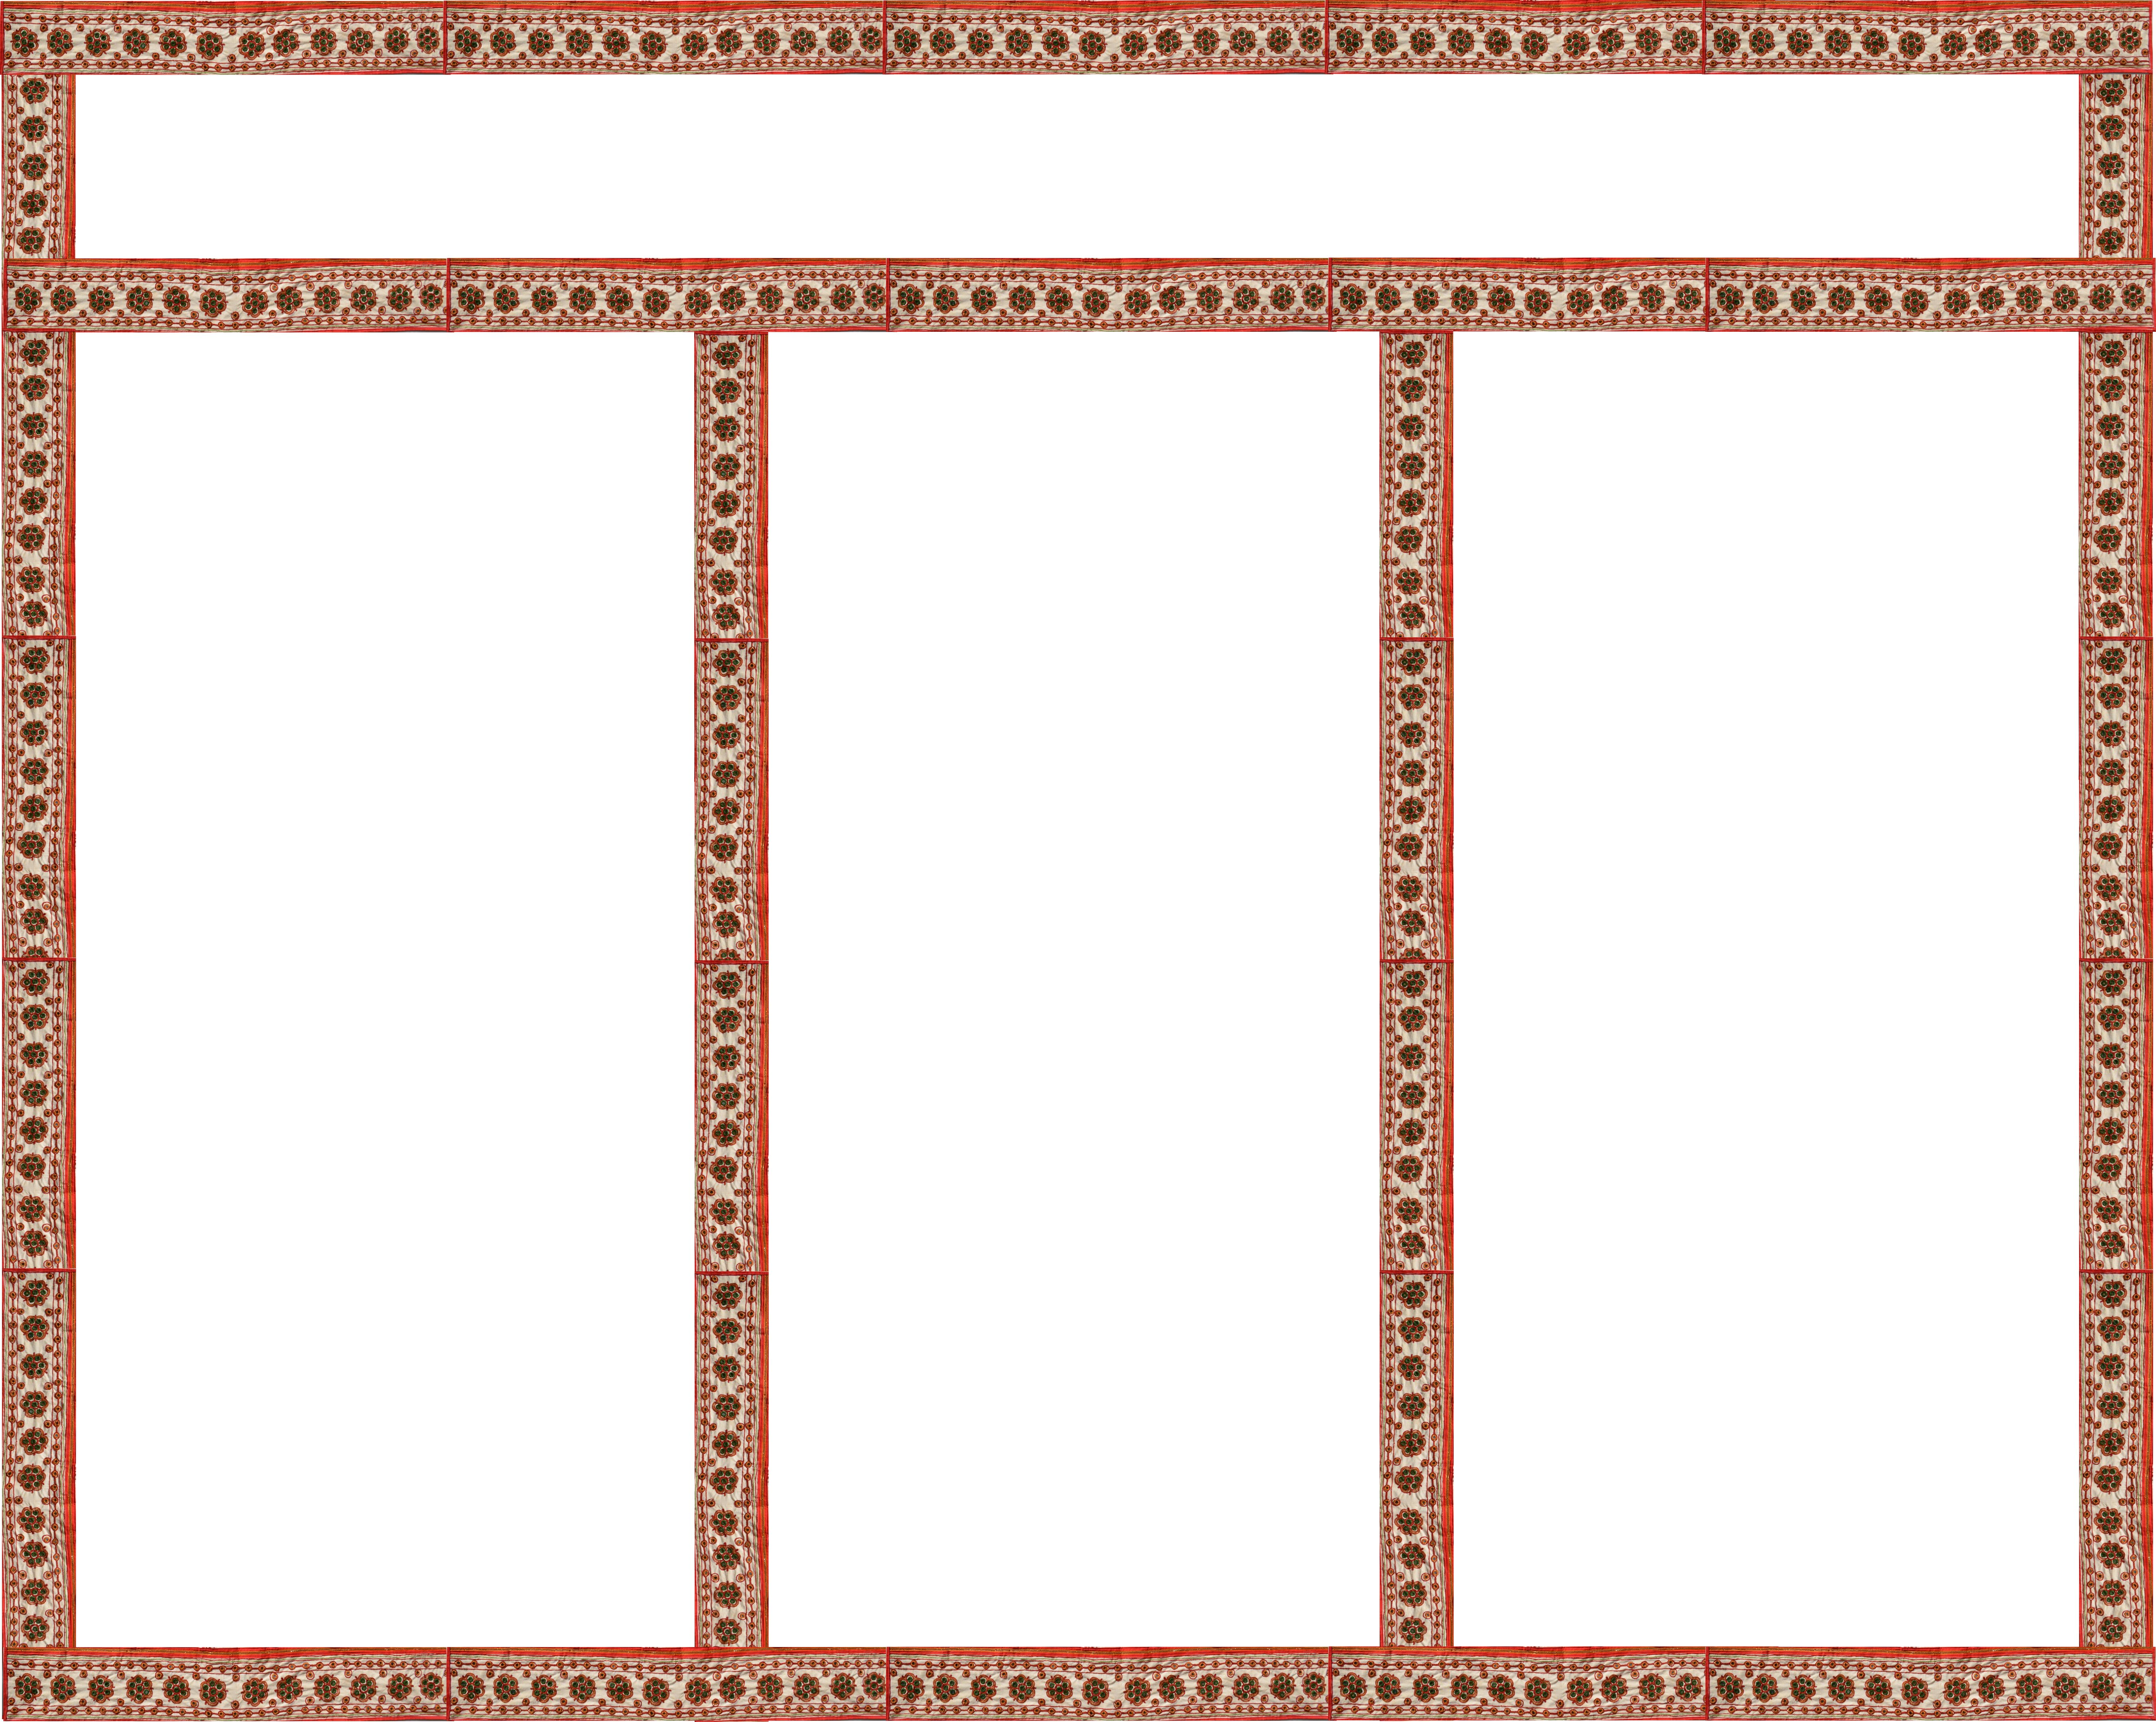
\includegraphics[width=\paperwidth,height=\paperheight]{./background/background.jpg}
    %};
%\end{tikzpicture}

\begin{tikzpicture}[remember picture, overlay]
    \centering
    \node[] (logo) at ([xshift=10cm, yshift=-5cm]current page.north west) { 
        
\includegraphics[height=6cm]{./images/NCBS-Logo.jpg}
    };

\node [
        align=center
        , shape = rectangle
        %, text width=0.7\paperwidth
        , inner sep=1cm
    %, execute at begin node=\setlength{\baselineskip}{2cm}] 
    ]
    (title) at ([yshift=-7cm]current page.north) {
        \textbf{ \sffamily
        \fontsize{72}{84}\selectfont { % here goes the title 
            Modeling Synaptic Switches Involved in Plasticity {\&}
            \textcolor{gray}{Protein Synthesis in Fragile X Syndrome}
        }
    }
    };

    \node[ align = center ] (authors) at ([yshift=-2cm]title.south) {
            \Huge
            Dilawar Singh $^1$, Upinder S. Bhalla $^1$, \textcolor{gray}{Nisha Ann Viswan $^1$, Aditi Bhattacharya$^2$
            , Melanie Stefan$^3$, Upinder S. Bhalla $^1$} \\
            \Large
            $^1$ National Center for Biological Sciences, Bangalore, $^2$ InStem, Bangalore
            , $^3$ University of Edinburgh, Edinburgh
        };

    \node [] (mooselogo) at ([xshift=-10cm,yshift=-5cm]current page.north east) {
        \includegraphics[height=5cm]{./images/moose_logo_tiny.png}
    };
    \node [] (gpl) at ([xshift=1cm,yshift=-0cm]mooselogo.south) {
        \TEXT{\textsc{An Open-Source Project}}
    };
\end{tikzpicture}


\vspace{0.04\paperheight}

%% Here goes the gallery.
%% This is summary of moose use cases.

\def\ghight{0.15\paperheight}
\def\gwidth{12cm}
\edef\figwidth{0.1\textwidth}

\begin{tikzpicture}
    \node[] (spineful_neuron) { 
        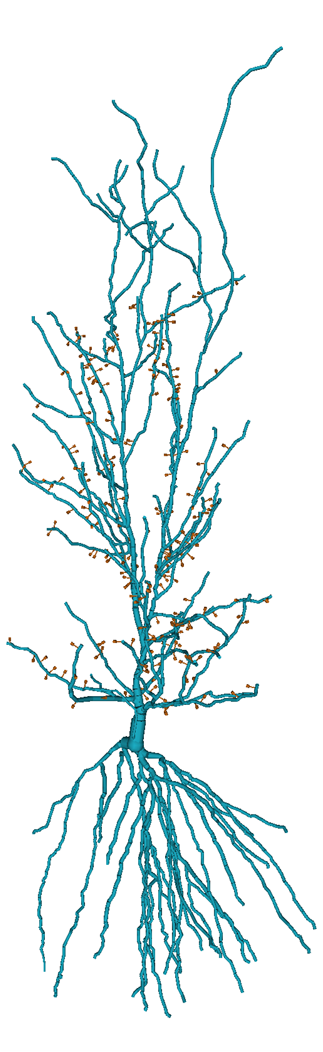
\includegraphics[height=\ghight]{./images/neuron_with_spine.png}
    };
\end{tikzpicture} \hfill %
\begin{tikzpicture}
    \node [] (moose_cell) {
        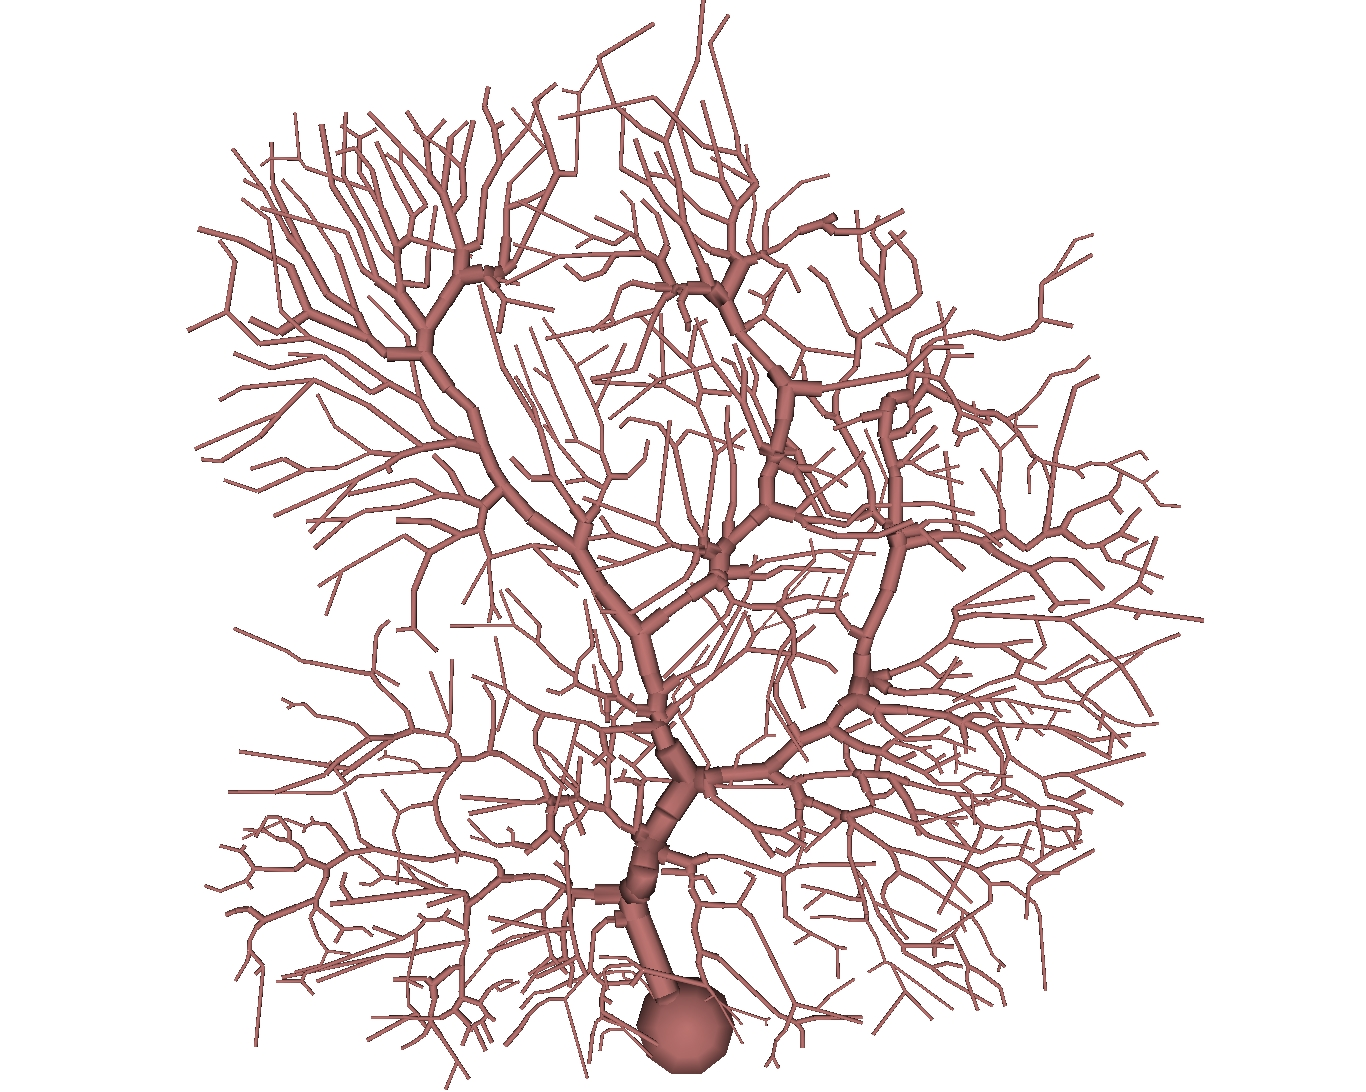
\includegraphics[height=\ghight]{./images/_1_7.jpeg}
    };
    %\node [text width=\figwidth,below=3.5cm] (captionA) {\CAPTION{Single Neuron Model}};
\end{tikzpicture} \hfill %
\begin{tikzpicture}
    % Now embed this neuron into a network.
    \node[] (subha1) {
        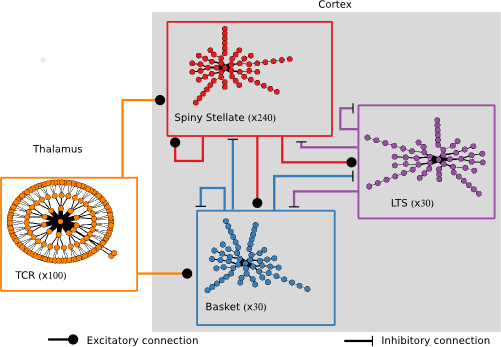
\includegraphics[height=\ghight]{./images/subha.png}
    };
\end{tikzpicture} \hfill %
\begin{tikzpicture}
    \node [] (subha) {
        \includegraphics[height=\ghight]{./images/reduced_model_pyramidical_cells.png}
    };
\end{tikzpicture} \hfill %
\begin{tikzpicture}
    \node[] (olfaction) {
        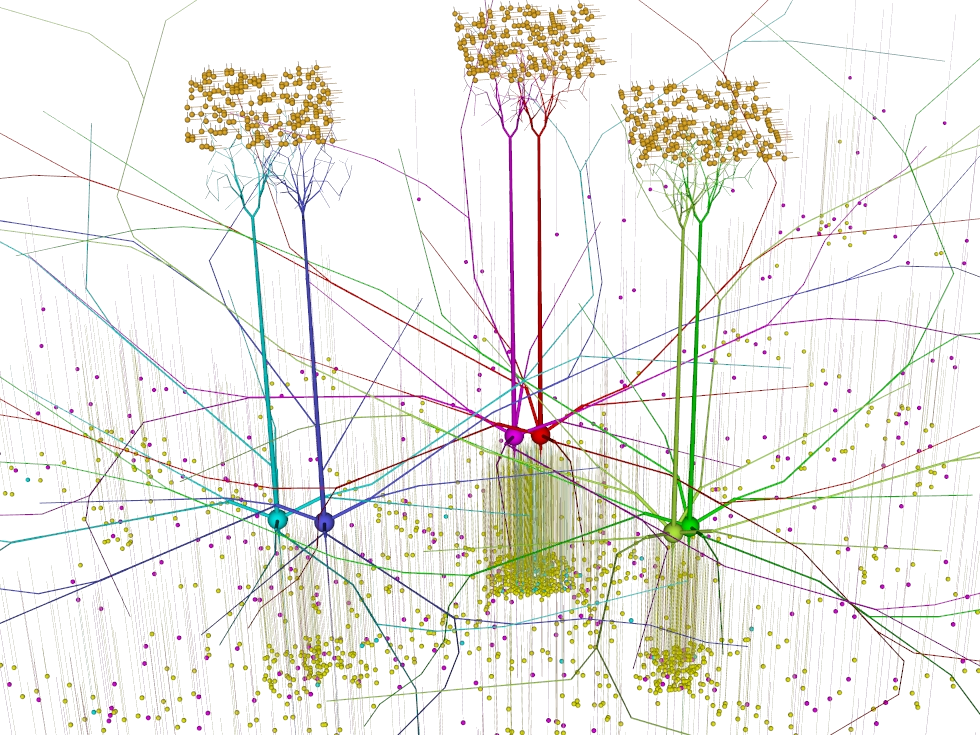
\includegraphics[height=\ghight]{./images/fullmodel_moogli.png}
    };
    %\node [text width=\figwidth, below=2.7cm] (captionB) {\CAPTION{Olfactory bulb model}};
\end{tikzpicture} \hfill %
\begin{tikzpicture}
    \node[] (projectb) {
        \includegraphics[height=\ghight]{./images/thalamocortical.png}
    };
\end{tikzpicture} \hfill %
\begin{tikzpicture}
    \node[] (chem_in_spine) { 
        \includegraphics[height=\ghight, width=20cm]{./images/psd_model.png}
    };
\end{tikzpicture} %



\vspace{0.03\paperheight}

j
%% Three columns
\setlength{\columnsep}{5cm}
\begin{multicols*}{3}
%% Column 1
\block{Synapse}{
    And what they do to memory
}

\block{CaMKII} {
    And why they are so silly 
}

%% column2 starts here
\SECTION{2.1 Modelling Memory}

\begin{tikzpicture}[
    spy using outlines={circle
        , magnification=10, connect spies
    }
    ]
    \centering
    \node [] (image) at (0,-1) {
        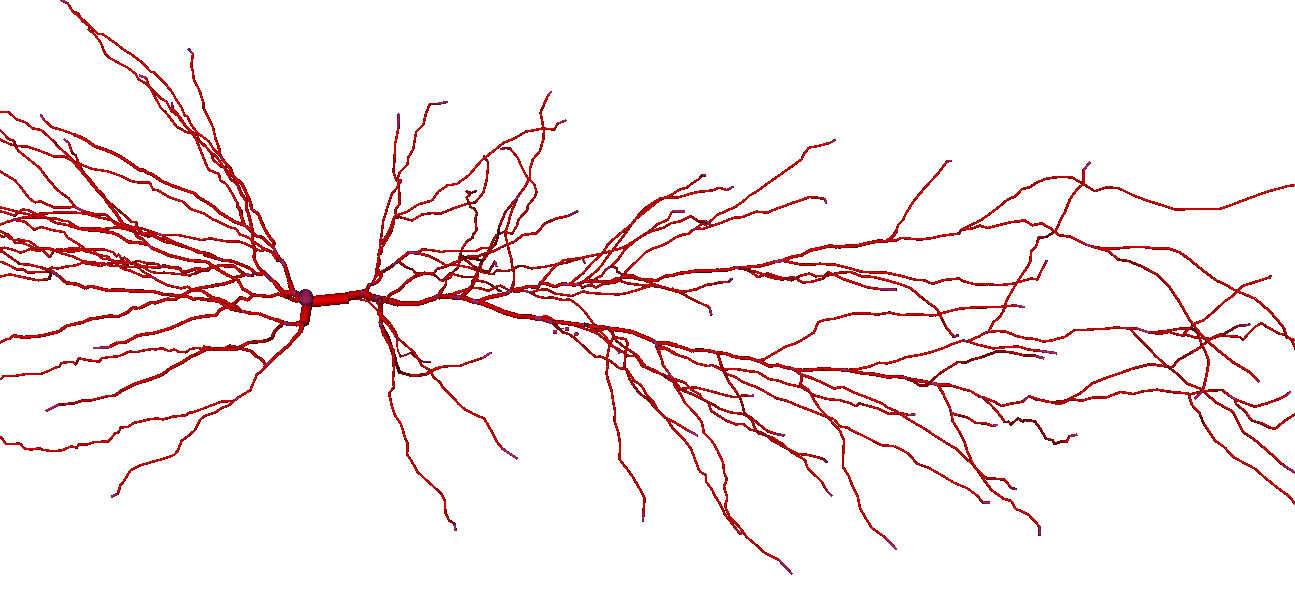
\includegraphics[scale=0.2,angle=-30]{./images/ca1_neuron.png}
    };

    \foreach \i in {-3,...,3}
    \foreach \j in {-3,...,3}
    {
        \node[fill=blue,opacity=0.3,thin,inner sep=0pt, minimum size=3mm,circle] (n\i\j) at (\i, \j) {};
    };

    \spy[blue, size=3cm] on (1.65, -1.5) in node[left] at (7,3);
    \node[below=4cm,text width=0.3\textwidth] {\CAPTION{A single detailed neuron is
            embedded in a network of simple cells}};

    %% Cool. Now create a 3d compartment model here.
    \begin{scope}[xshift=11cm, yshift=3cm
        , compartment/.style={cylinder
            , draw
            , cylinder uses custom fill
            , cylinder end fill = red!35
            , cylinder body fill = red!40
            , inner sep = 3mm
            , minimum height = 1cm
            , minimum width = 1cm 
        }
        , spine/.style={cylinder 
            , fill = blue!20
            , inner sep=1mm
            , minimum height=1mm
            , minimum width=3mm
        }
        , branch/.style={cylinder
            , draw
            , cylinder uses custom fill
            , cylinder end fill = red!35
            , cylinder body fill = red!40
            , minimum height = 1.5cm
            , minimum width = 0.5cm
            , inner sep = 1mm
        }
        ]

        \node[compartment] (c1) {};
        \node[compartment] (c2) at (c1.east) {};
        \node[compartment] (c3) at (c2.east) {};

        \node[branch,rotate=45] (b1) at ([xshift=4mm,yshift=2mm]c3.before top) {};
        \node[branch,rotate=-45] (b2) at ([xshift=1mm, yshift=-7mm]c3.base east) {};

        % Spines
        \node[spine, inner sep=1mm, rotate=135] (s11) at (b1.north east) {};
        \node[spine, inner sep=1mm, rotate=135] (s12) at ([xshift=3mm]b1.south east) {};

        \node[spine, inner sep=1mm, rotate=45] (s21) at (b2.north east) {};
        \node[spine, inner sep=1mm, rotate=45] (s22) at ([xshift=-3mm]b2.south east) {};

    \end{scope}

    %% Scope to draw chemisty 
    \begin{scope}

        \node[] (chemical) at ([yshift=-6cm]c2.south) {
            \includegraphics[width=0.35\textwidth, trim=5mm 5mm 5mm 5mm, clip]{./images/chemical_reactions.png}
        };

        %%  
        \node [above] (chemicallabel) at ([yshift=-2cm]c1.south) {\LARGE{
                Chemical models}};

        \draw[o-o] (c1.center) to [bend right] (chemicallabel.center);

        %% Add transportation model.
        \node[] (transport) at ([xshift=7cm,yshift=-3cm]s12.north) {
            \includegraphics[width=0.3\textwidth]{./images/transport_mechanism.png}
        };

        \node[] (tlabel) at ([xshift=0.5cm, yshift=0cm]transport.north) {\LARGE{Trafficking
                models}};

        \draw[o-o] (s21.center) to [bend left] (tlabel) ;

    \end{scope}
\end{tikzpicture}


\vspace{1cm}
\begin{tikzpicture}
    \node[] (label) at ([xshift=-20cm]tlabel) {
        \CAPTION{\hspace{12cm} Neighbouring spines are modified differently}
    };
\end{tikzpicture}

%% memory results by upi
\begin{tikzpicture}
    \node[] (resultb) {
        \includegraphics[width=0.5\textwidth]{./images/spike_raster.png}
    };
\end{tikzpicture} \hfill %
\begin{tikzpicture}
    \node[] (resultA) {
        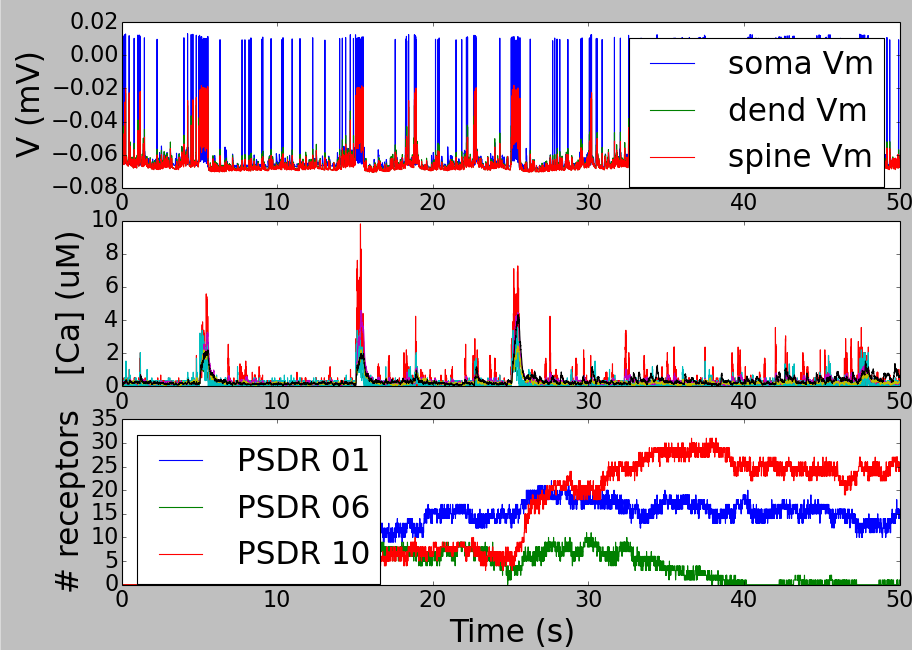
\includegraphics[width=0.5\textwidth]{./images/timeseries.png}
    };
\end{tikzpicture}


\begin{Figure}

\SECTION{2.2 Modelling Olfactory Bulb}
\centering
\begin{tikzpicture}
    \node[] (aditya) {
        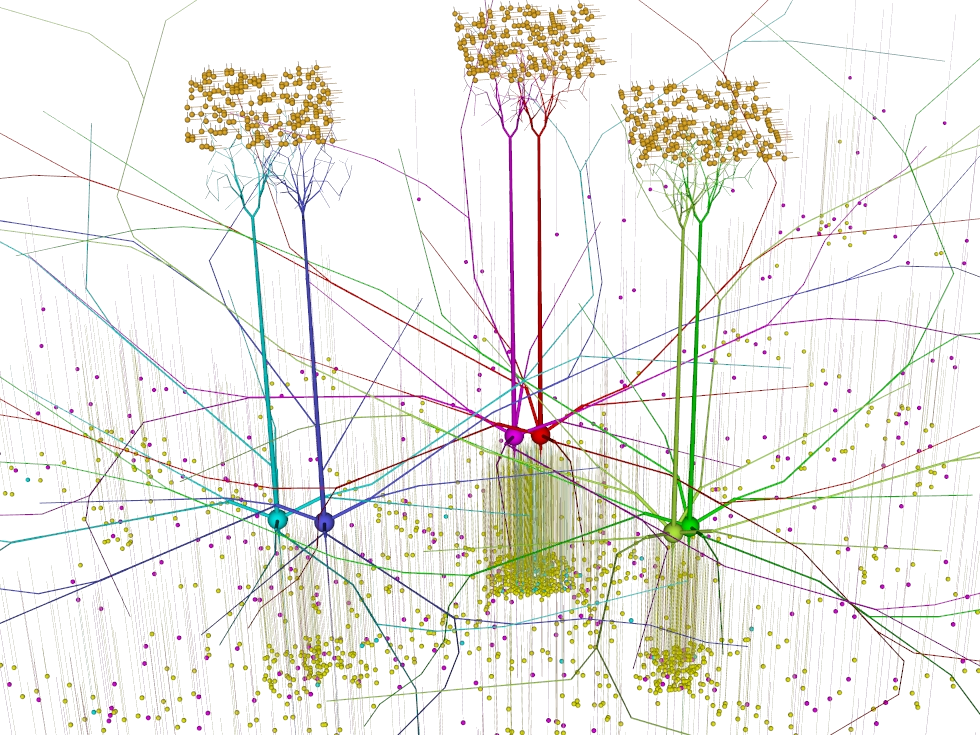
\includegraphics[width=\textwidth]{./images/fullmodel_moogli.png}
    };
\end{tikzpicture}
\vspace{1cm}

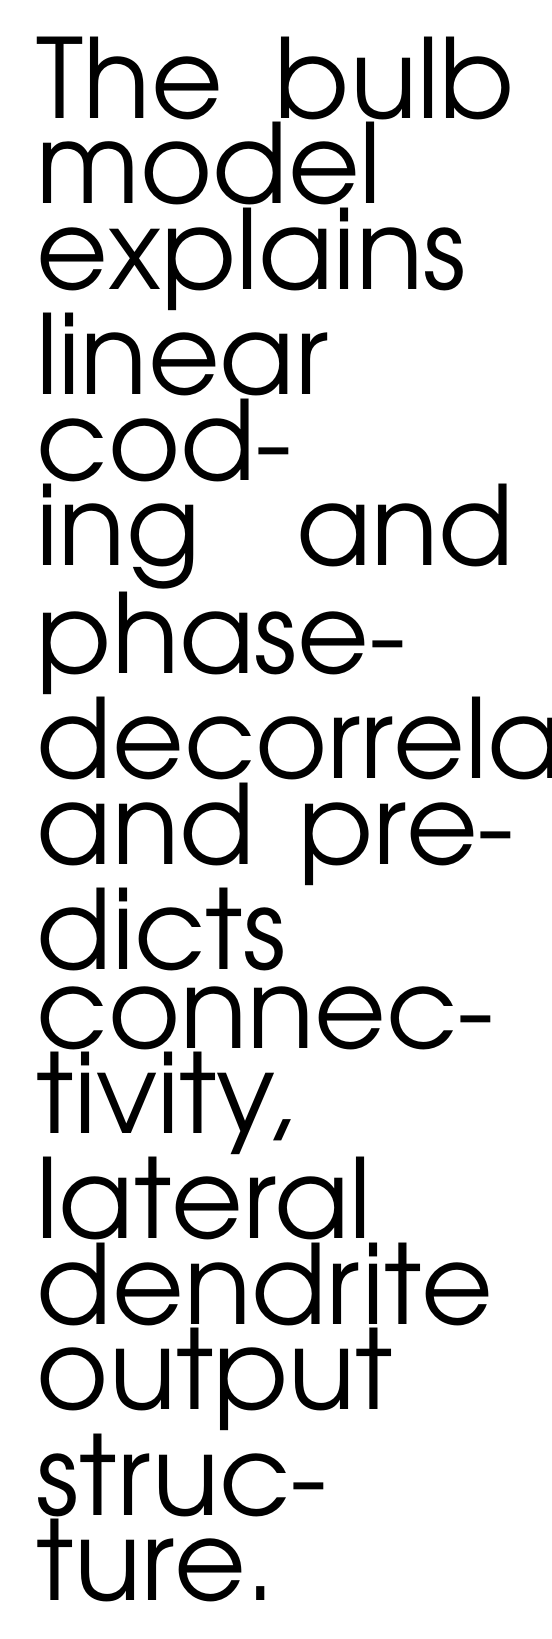
\begin{tikzpicture}
    \node[] (caption) {
        \begin{minipage}{0.5\textwidth}
            \TEXT{
                The bulb model explains linear coding and phase-decorrelation and
                predicts connectivity, lateral dendrite output structure.} 
        \end{minipage}
    };
\end{tikzpicture} \hfill%
\begin{tikzpicture}
    \node[] (result) {
        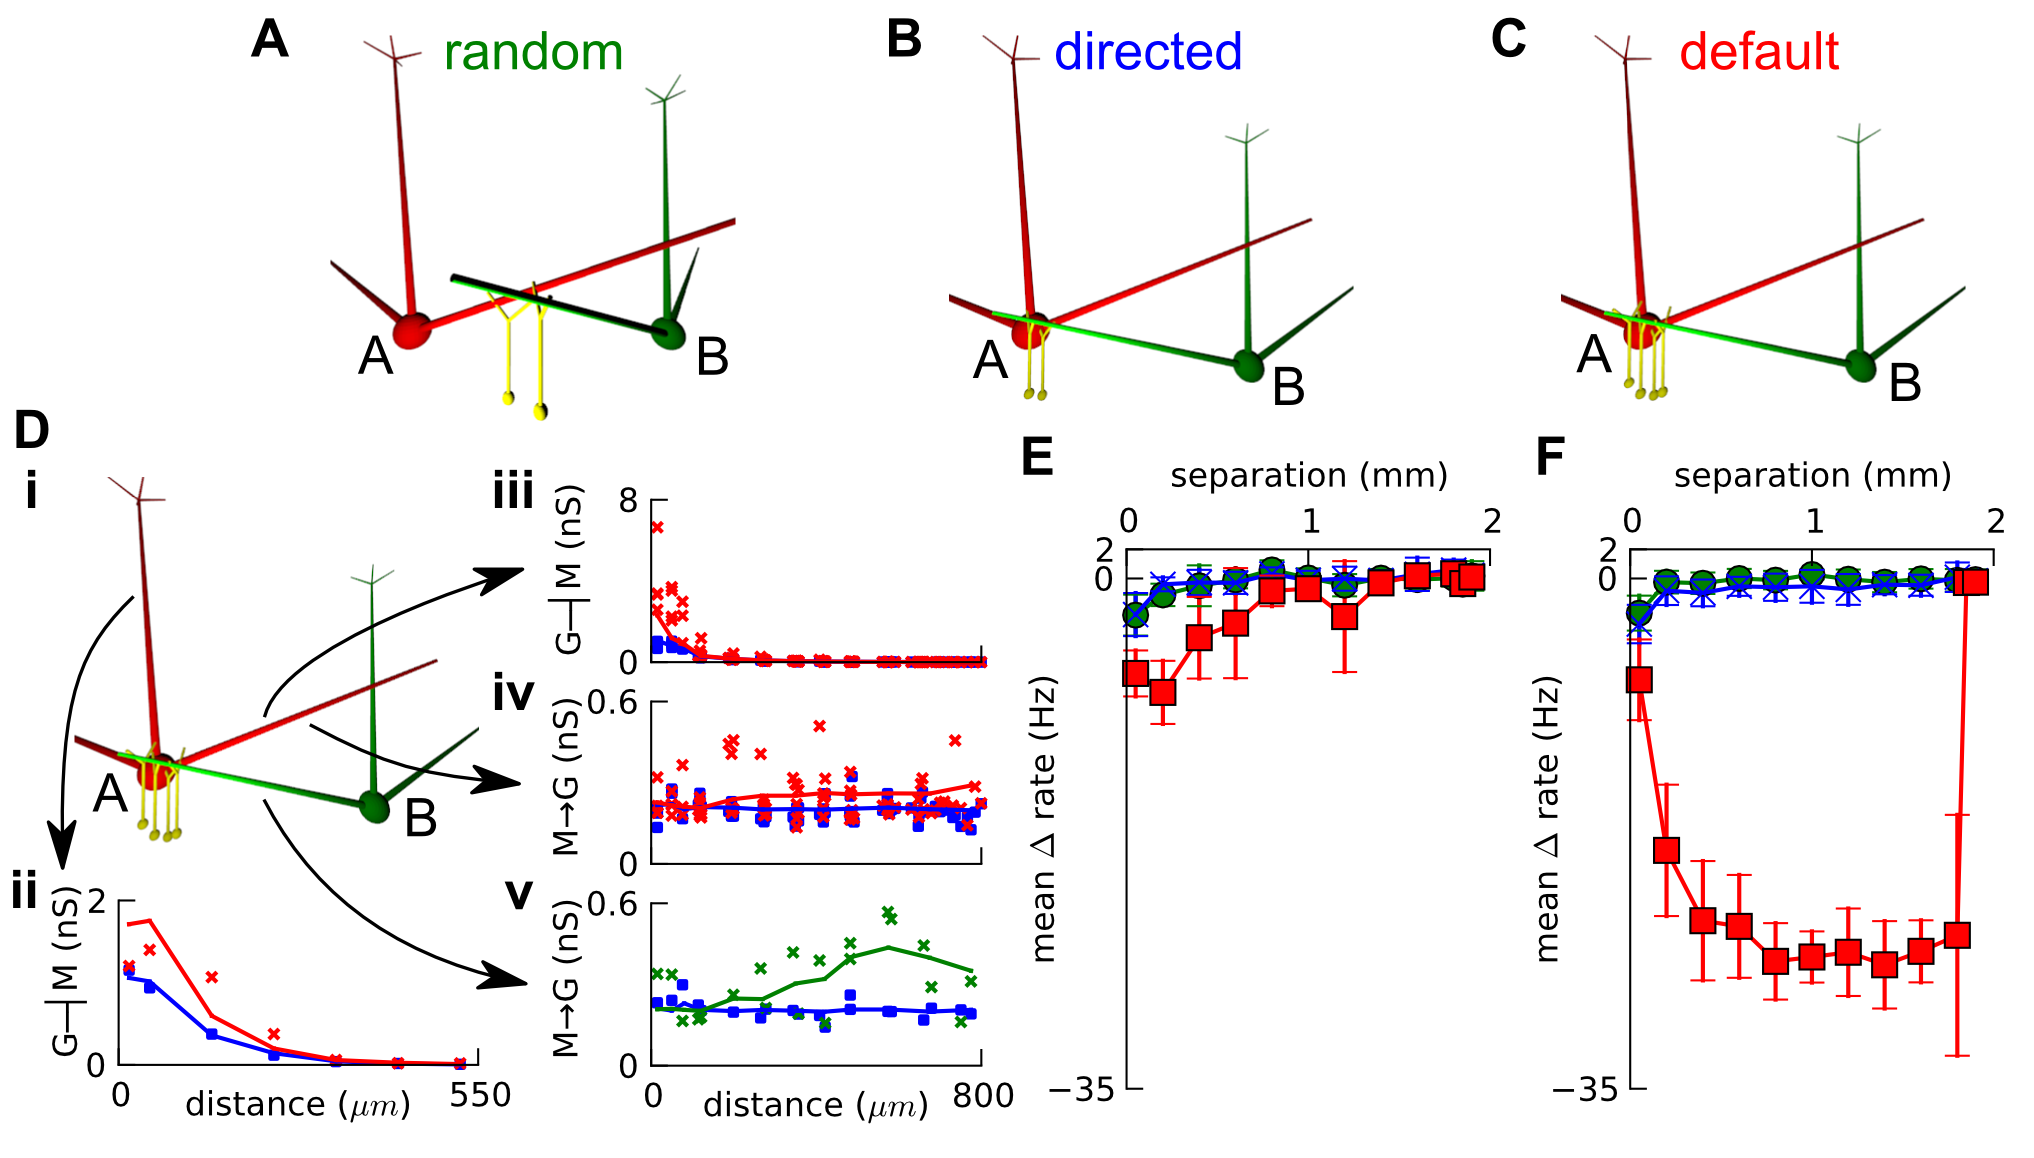
\includegraphics[width=0.45\textwidth]{./images/aditya_work.png}
    };
\end{tikzpicture}

%% One more model here.
\raggedright
\SECTION{2.3 Modelling Cortex}

\TEXT{\bf Predicts:}

\centering
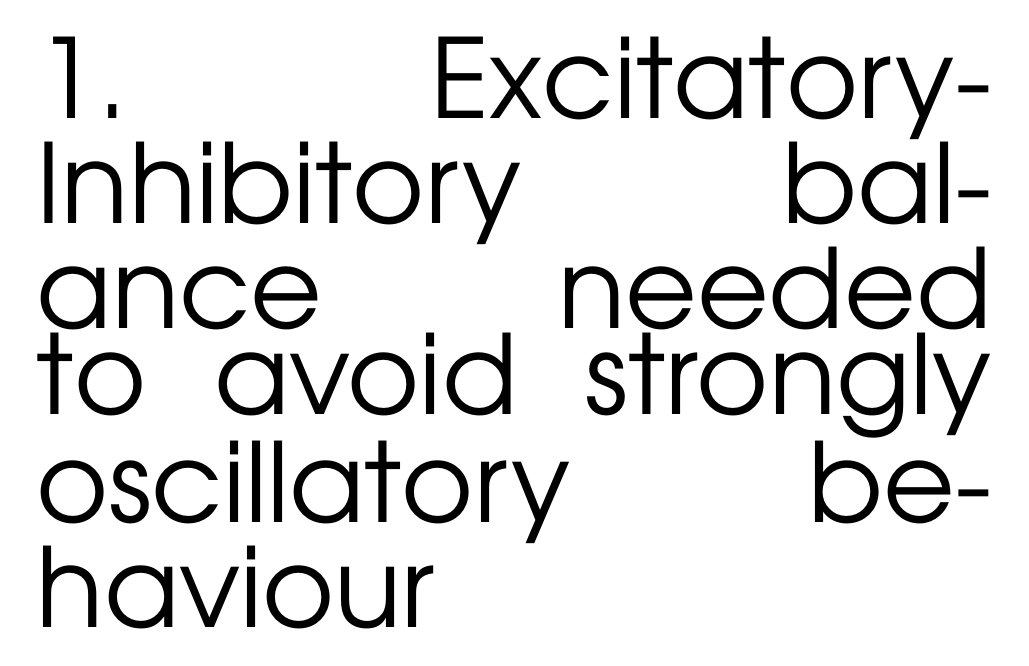
\begin{tikzpicture}
    \node [] (label) {
        \begin{minipage}{\textwidth}
            \TEXT{1. Excitatory-Inhibitory balance needed to avoid strongly oscillatory
                behaviour}
        \end{minipage}
    };
\end{tikzpicture}

\begin{tikzpicture}
    \node [] (label) {
        \begin{minipage}{\textwidth}
            \TEXT{2. Many weakly connected basket cells better at suppressing
                oscillations}
        \end{minipage}
    };
\end{tikzpicture}

\vspace{-1cm}
\begin{tikzpicture}
    \node[] (robust) {
        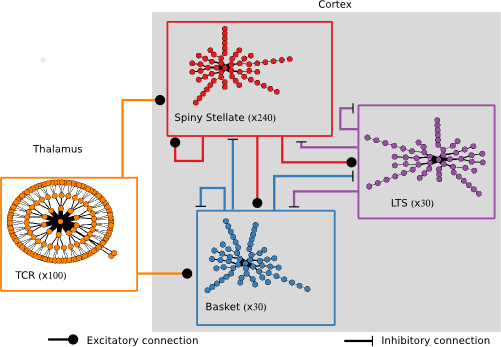
\includegraphics[width=0.9\textwidth]{./images/subha.png}
    };
\end{tikzpicture}

\end{Figure}


\begin{Figure}

    \HEADING{MOOSE makes multiscale modeling easier}

    \TEXT{Rdesigneur (\textbf{R}eaction-\textbf{D}iffusion and
        \textbf{E}lectrical \textbf{SIG}naling in \textbf{NEUR}on) class makes it
        easier to mix models across scales:}
        
    \TEXT{Following databases/models are supported}
    \begin{itemize}
        \item \TEXT{Neuron morphology and network, \texttt{NeuroMorpho (SWC),
                    NeuroML}}
        \item \TEXT{Chemical pathways, Reaction diffusion models, \texttt{System
                Biology Markup Language (SBML), DOQCS, KKIT}}
        \item \TEXT{Ion-channels models \texttt{channelpedia, OpenSourceBrain}}
    \end{itemize}
    
    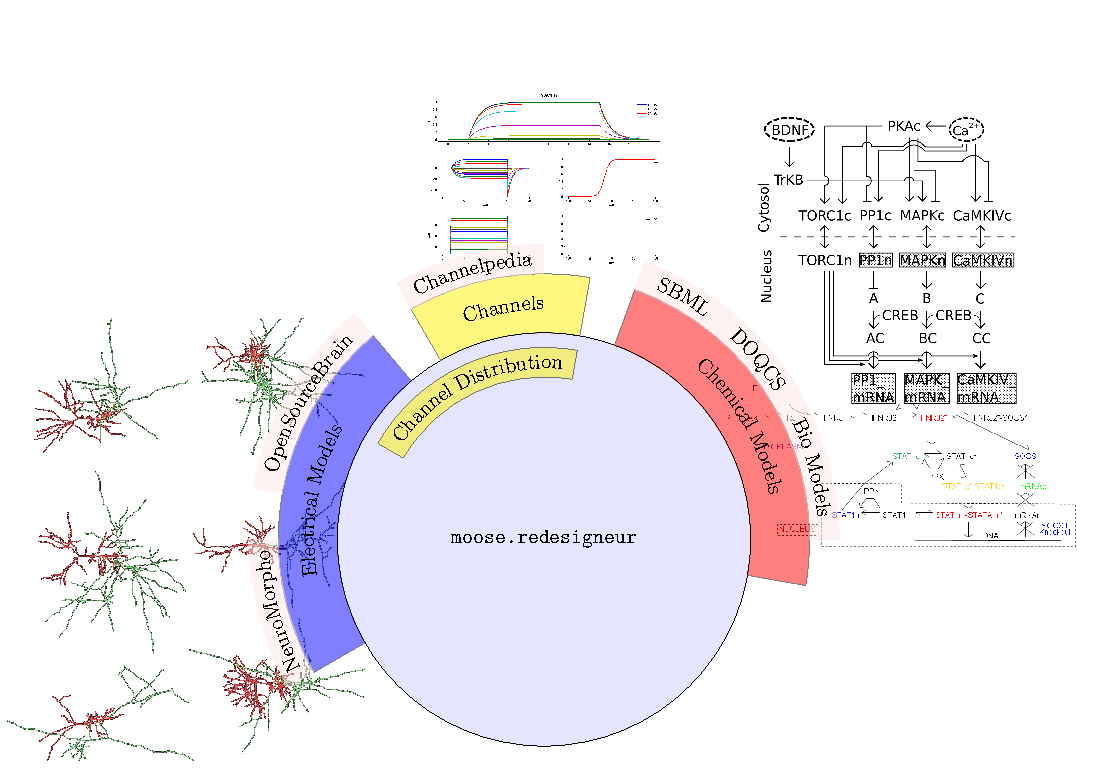
\includegraphics[width=\textwidth]{./_images/rdesigneur.pdf}

    \HEADING{Supported Platforms}

    \TEXT{Packages are available for all major Linux flavors}
    { 
        \includegraphics[width=\textwidth]{./_images/supported_platforms.png}
        \includegraphics[width=\textwidth]{./_images/supported_platforms1.png}
    }

    \HEADING{Summary}
    \begin{itemize}

        \item \TEXT{Designed to be multiscale from the onset. Integrate many
                scales of neuronal data with basic physical/chemical
                principles.}

        \item \TEXT{Rdesigneur makes it easy to mix chemical, electrical and
                channel models in \MOOSE}

        \item \TEXT{Easily scriptable via Python. GUI/3D visualization support}
        \item \TEXT{Packages are available for Linux/MaxOSX. Python-scripting
                interface builds on Windows under Cygwin}

    \end{itemize}

    \TEXT{Source code {\bf https://github.com/BhallaLab/moose}. Packages and
        documentation {\bf http://moose.ncbs.res.in}}

\end{Figure}





\end{multicols*}

\end{document}
